\begin{center}
    \section*{\fontsize{20}{20}\selectfont Chapter 3}
\end{center}
\vspace{10mm}
\section{Research Methodology}

This chapter explains how we built the potato leaf disease detection system. We first give the five-stage framework. Then we describe the leak-aware 5-class dataset and the preprocessing steps. After that we explain the design and training of our main model, a small MobileNetV2, and of the three comparison models (MultiNet-V3 Ensemble, InceptionV3 and NASNetMobile). The chapter ends with the Grad-CAM, Google Gemini and FastAPI/React web application modules.

\subsection{Proposed Framework}
We wanted high accuracy, a model under 9~MB, and an interface that is easy to understand. To get there, the system is split into five linked stages, shown in Figure~\ref{fig:workflow}:
\begin{enumerate}
    \item \textbf{Dataset audit and leak-aware splitting.} We audit all 2,321 field photos in five potato classes. 64-bit perceptual difference hashing ($\text{dHash} \le 10$) groups them into 2,283 groups without duplicates. \texttt{StratifiedGroupKFold} (80:10:10) then splits the groups into separate training, validation and test sets.
    \item \textbf{Preprocessing, augmentation and class balancing.} Images are resized to the input size of each model ($224 \times 224 \times 3$, or $299 \times 299 \times 3$ for InceptionV3). During training they get leaf-like geometric and color changes on the fly. Inverse-frequency class weights, capped at $3.0$, reduce the effect of the uneven classes.
    \item \textbf{Training the small model and the benchmarks.} Our MobileNetV2 (2.26M parameters, 8.64~MB) is trained in two stages with AdamW and frozen BN on two NVIDIA Tesla T4 GPUs. The three other models (MultiNet-V3 Ensemble, InceptionV3 and NASNetMobile) are tested in the same way.
    \item \textbf{Checked evaluation, TTA and Grad-CAM.} Each candidate checkpoint is reloaded from disk to confirm that export does not change its output ($0.00 \times 10^{0}$ maximum probability difference). We then score it with single-pass and 4-view Test-Time Augmentation (TTA), and inspect it with Grad-CAM heatmaps.
    \item \textbf{Web application and bilingual Gemini advice.} The checked 8.64~MB \texttt{.keras} model runs behind a FastAPI backend and a React frontend (\url{https://potato.mamunlab.com/}). The app supports camera capture, batch analysis, PDF/CSV export, Grad-CAM overlays and Google Gemini chat in English and Bengali.
\end{enumerate}

\begin{figure}[htbp]
\centering
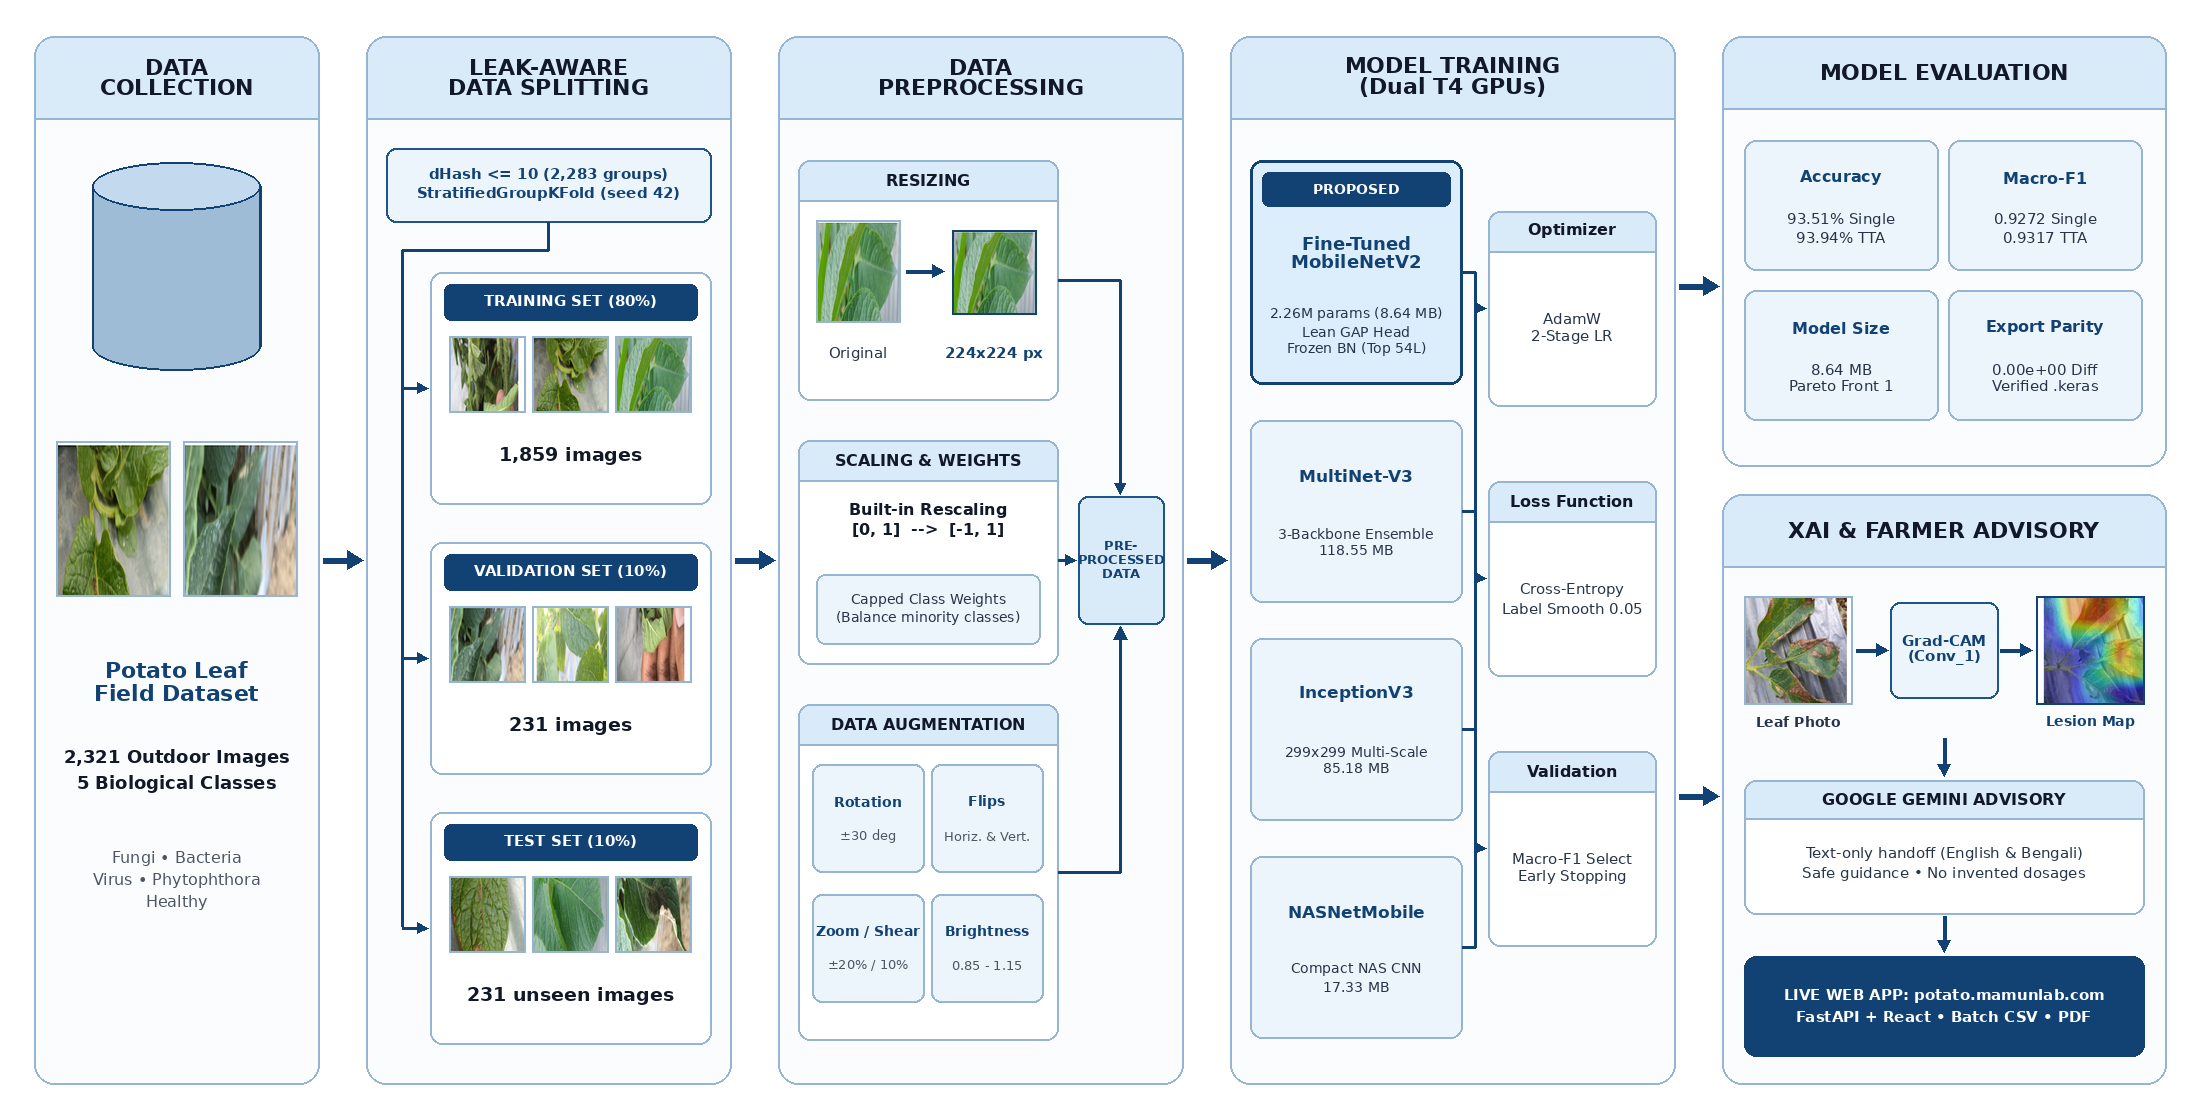
\includegraphics[width=0.98\textwidth]{image/workflow.png}
\caption{End-to-end methodology and system architecture of the compact explainable potato leaf disease detection and farmer advisory framework.}
\label{fig:workflow}
\end{figure}

Before the full run, we checked that the project was feasible in three ways.

\textit{Technical.} Training runs in a repeatable way on two NVIDIA Tesla T4 GPUs on Kaggle, with TensorFlow~2.20--2.21, Keras~3.13.2 \cite{abadi2016tensorflow} and \texttt{tf.distribute.MirroredStrategy}. We use only built-in Keras layers and no custom Lambda layers, so the same \texttt{.keras} file loads both in training and in the FastAPI server.

\textit{Operational.} The exported classifier is only 8.64~MB. The web backend therefore starts fast, uses little memory and answers quickly when a farmer uploads a photo or takes one with a phone camera. No farming expertise is needed to use it.

\textit{Economic.} All deep learning, vision and web tools we use are open source. Training ran on free Kaggle GPU hours. The Google Gemini model (\texttt{gemini-3.1-flash-lite}) receives only a short text summary of the result, not the image, so the running cost of the advice stays low.

\subsection{Dataset Analysis and Project Requirements}
We use a curated 5-class potato leaf dataset (\texttt{potato-disease-dataset-03}) built from field photos taken in uncontrolled conditions \cite{shabrina2024novel}. We kept the five main classes: Bacteria, Fungi, Healthy, Phytopthora and Virus. (Phytopthora is the folder name used in the source data for \textit{Phytophthora} late blight, and we kept that spelling.) Classes for pests and nematodes had very few images, so we left them out. The real field clutter stays in the photos: soil, shadows, plastic mulch, hands and overlapping leaves.

Table~\ref{tab:class_dist} shows the numbers. There are 2,321 RGB field images. The imbalance is moderate, $3.66:1$, between the largest class (\textit{Fungi}, 729 images, 31.41\%) and the smallest (\textit{Healthy}, 199 images, 8.57\%). The class index order (\texttt{Bacteria}, \texttt{Fungi}, \texttt{Healthy}, \texttt{Phytopthora}, \texttt{Virus}) is fixed in code. All four model notebooks and the FastAPI backend use this same order, so the indices never depend on how the file system lists the folders.

\begin{table}[htbp]
\caption{Dataset Classes, Image Counts, and Capped Training Class Weights (5-Class Contract)}
\label{tab:class_dist}
\begin{center}
\begin{tabularx}{0.95\textwidth}{| c | l | X | c | c | c |}
\hline
\textbf{Index} & \textbf{Folder Label} & \textbf{Display Name} & \textbf{Images} & \textbf{Share (\%)} & \textbf{Norm.\ Weight} \\
\hline
0 & \texttt{Bacteria} & Bacterial Disease & 566 & 24.39\% & 0.6546 \\
\hline
1 & \texttt{Fungi} & Fungal Disease & 729 & 31.41\% & 0.5169 \\
\hline
2 & \texttt{Healthy} & Healthy & 199 & 8.57\% & 1.8857 \\
\hline
3 & \texttt{Phytopthora} & Phytophthora & 306 & 13.18\% & 1.2238 \\
\hline
4 & \texttt{Virus} & Viral Disease & 521 & 22.45\% & 0.7190 \\
\hline
\multicolumn{3}{|l|}{\textbf{Total (5-Class Contract)}} & \textbf{2,321} & \textbf{100.00\%} & \textbf{Mean = 1.0000} \\
\hline
\end{tabularx}
\end{center}
\end{table}

\subsubsection{Data Collection, Leak-Aware Splitting, and Preprocessing}
Field datasets often hold several burst frames or crops of the same leaf. With a simple random split, almost identical copies can end up in both the training and the test set, and the test score looks better than it is. To stop this in every experiment, we convert each image to a 64-bit grayscale perceptual difference hash (\texttt{dHash}, $9 \times 8$ Lanczos downsample). Two images are joined with union-find when the Hamming distance between their hashes is $\text{dHash} \le 10$. This gives \textbf{2,283 unique groups} from the 2,321 images.

The groups are then split in two steps with \texttt{StratifiedGroupKFold} (\texttt{random\_state = 42}). A 10-fold outer split picks the test set, and a 9-fold inner split picks the validation set. The result is an 80:10:10 split of \textbf{1,859 training}, \textbf{231 validation} and \textbf{231 unseen test} images. Assertions in the code confirm that no group appears in two sets. Every notebook uses the same hashing and the same seed, so all four models are tested on \textbf{the same 231 test images}.

Preprocessing and augmentation follow three rules.

\textit{Resizing and scaling.} The data generator resizes RGB images to $224 \times 224 \times 3$ ($299 \times 299 \times 3$ for InceptionV3) and divides the pixels by $255.0$ to get values in $[0, 1]$. The FastAPI server does the same. Inside our MobileNetV2, a built-in \texttt{layers.Rescaling(scale=2.0, offset=-1.0)} layer maps $[0, 1]$ to the $[-1, 1]$ range that the pretrained MobileNetV2 expects. Because this step is part of the model, it is saved inside the exported \texttt{.keras} file.

\textit{Augmentation.} The validation and test generators only rescale. The training generator adds random rotation ($\pm 30^\circ$), horizontal and vertical shifts ($\pm 15\%$), shear ($10\%$), zoom ($\pm 20\%$), horizontal and vertical flips (a leaf has no fixed up or down), and brightness changes ($[0.85, 1.15]$) to imitate outdoor light \cite{shorten2019survey}.

\textit{Class weights.} We compute inverse-frequency weights $w_c = N_{\text{train}} / (C \cdot n_c)$, cap them at $3.0$ and scale them to a mean of $1.0$ (Table~\ref{tab:class_dist}). This keeps the small classes (\textit{Healthy}, \textit{Phytopthora}) from being ignored, while the gradients stay stable.

\subsubsection{Feature Selection and Representation}
Classic pipelines used color histograms or GLCM/SIFT features \cite{alhiary2011fast, arivazhagan2013detection}. In our framework the pretrained convolutional backbone selects the features itself, layer by layer. In MobileNetV2 the early inverted-residual blocks react to local color edges and spot borders. The deeper $14 \times 14$ and $7 \times 7$ blocks (\texttt{block\_11} to \texttt{Conv\_1}) capture higher-level patterns, such as dead tissue texture, the water-soaked edges of late blight and viral mosaic. \texttt{GlobalAveragePooling2D} (GAP) turns the final $7 \times 7 \times 1280$ tensor into a 1,280-value vector and adds no parameters. GAP also acts as a regularizer. Its output goes to the softmax classifier, and the same feature map is used for Grad-CAM.

\subsubsection{Software and Hardware Project Requirements}
\textit{Functional requirements.} The system accepts RGB potato leaf photos (JPG/PNG, up to 10~MB) by upload or camera. It keeps the fixed 5-class index order. It returns the predicted class, the confidence and the full probability list, and draws a Grad-CAM overlay. It can screen 12 images at once and export CSV/PDF. It offers Gemini chat in English and Bengali, with safety notes.

\textit{Non-functional requirements.} Accuracy and macro-F1 should be above 90\% on unseen data without leakage. The model should stay under 10~MB so it is cheap to serve on the web or on an edge device. The exported model must give the same output as the trained one ($\Delta p \le 10^{-3}$). The code should stay modular so the model can be converted to TFLite for phones later.

\textit{Hardware requirements.} Training uses two NVIDIA Tesla T4 GPUs in the cloud (16~GB VRAM each, two synchronized replicas). Inference with FastAPI runs well on a normal CPU server, a laptop or an edge device with at least 4~GB RAM.

\subsection{Algorithm and Model Analysis}

\subsubsection{Proposed Compact Model: Fine-Tuned MobileNetV2}
Our main model uses \textbf{MobileNetV2} pretrained on ImageNet \cite{sandler2018mobilenetv2}. We kept the classifier head very small, because there are only 1,859 training images and we wanted the full model to stay at \textbf{8.64~MB} (2,264,389 parameters):
\begin{equation}
\begin{aligned}
\text{Input }(224,224,3) &\xrightarrow{\text{Rescaling}} \text{MobileNetV2 (154 layers)} \\
&\xrightarrow{\text{GAP}} \mathbb{R}^{1280} \xrightarrow{\text{Dropout}(0.25)} \text{Dense}(5, \text{Softmax}).
\end{aligned}
\end{equation}
The head adds only \textbf{6,405 parameters} (25.02~KB) on top of the 2,257,984 parameters of the backbone. We did not want to make the model any larger. Instead, we made four changes to the training of a first, unoptimized baseline:
\begin{enumerate}
    \item \textbf{Restore the best Stage~1 weights.} We first train the head for 10 epochs with the backbone frozen ($\text{LR} = 10^{-3}$). Before unfreezing, we reload the Stage~1 checkpoint with the best \texttt{val\_macro\_f1}. Fine-tuning then starts from the best head weights, not from the last epoch.
    \item \textbf{Keep Batch Normalization frozen during fine-tuning.} In Stage~2 (up to Epoch~60) we open the top 54 backbone layers (\texttt{block\_11} to \texttt{Conv\_1}) for training. Every \texttt{BatchNormalization} layer in the backbone stays frozen (\texttt{layer.trainable = False} and \texttt{training = False}). This leaves 36 convolutional and depthwise layers trainable. It also stops the batch-statistics shock that, in our first baseline, made the validation loss jump from $0.83 \rightarrow 2.63$.
    \item \textbf{AdamW, gradient clipping and less label smoothing.} We replaced Adam with \texttt{AdamW} ($\text{weight\_decay} = 10^{-4}$, $\text{clipnorm} = 1.0$) \cite{loshchilov2019decoupled} and lowered label smoothing from $\epsilon = 0.10 \rightarrow 0.05$. This regularizes the weights better and makes the model separate \textit{Phytophthora} and \textit{Fungi} lesions, which look alike, more clearly.
    \item \textbf{4-view Test-Time Augmentation (TTA).} At test time, the 8.64~MB model can average its softmax output over four fixed views: the original, a horizontal flip, a vertical flip and both flips. This raises macro-F1 and adds no parameters.
\end{enumerate}

\subsubsection{Comparative Benchmark Architectures}
To judge the accuracy and size of our MobileNetV2 fairly, we built three other models with one shared two-stage transfer-learning setup. All three use \texttt{Head LR = 3e-4}, \texttt{Fine-tune LR = 3e-5} and the head \texttt{GAP $\rightarrow$ Dropout $\rightarrow$ Dense(256) $\rightarrow$ BN $\rightarrow$ Swish $\rightarrow$ Dropout $\rightarrow$ Softmax(5)}. They use the same 5-class leak-aware split and the same two T4 GPUs.

\textit{MultiNet-V3 Ensemble (31,077,492 params, 118.55~MB).} This is a large three-backbone ensemble. It joins ImageNet-pretrained \textbf{EfficientNetB0} \cite{tan2019efficientnet} (4.05M), \textbf{MobileNetV2} \cite{sandler2018mobilenetv2} (2.26M) and \textbf{ResNet50} \cite{he2016deep} (23.59M). We avoided Keras Lambda layers so the \texttt{.keras} file loads safely anywhere. For MobileNetV2 the input is scaled with a built-in \texttt{Rescaling} layer. For ResNet50, the BGR channel swap and ImageNet mean subtraction are done by a frozen $1 \times 1$ \texttt{Conv2D} layer (12 non-trainable parameters). The three $7 \times 7$ outputs are joined along the channel axis into \texttt{ensemble\_\allowbreak spatial\_\allowbreak features} $(7, 7, 4608)$, which then goes to GAP and the dense head.

\textit{InceptionV3 (22,329,637 params, 85.18~MB).} This model works at a larger input size ($299 \times 299 \times 3$) with factorized multi-scale Inception modules \cite{szegedy2016rethinking}. A 2,048-channel GAP vector feeds the shared Swish head (526,341 head parameters).

\textit{NASNetMobile (4,542,617 params, 17.33~MB).} This model uses normal and reduction cells found by neural architecture search \cite{zoph2018learning}. Its $7 \times 7 \times 1056$ output goes to the shared head (272,389 head parameters).

\subsubsection{Training Optimization, Checkpointing, and Export Verification Protocol}
If we watched only the validation loss, we could pick a checkpoint that predicts mostly the largest class. So every notebook has a custom \texttt{MacroF1Callback}. It computes the exact validation \textbf{macro-F1} after each epoch, and this value drives \texttt{ModelCheckpoint}, \texttt{ReduceLROnPlateau} and \texttt{EarlyStopping}. After training, the candidate checkpoints (\texttt{head-checkpoint}, \texttt{fine-tune-checkpoint} and the reloaded \texttt{final-epoch}) are loaded from disk outside \texttt{MirroredStrategy}, so they behave exactly as they will on a single serving device. Before export, three automatic checks must pass: \texttt{predicts\_\allowbreak more\_\allowbreak than\_\allowbreak one\_\allowbreak class}, \texttt{macro\_\allowbreak f1\_\allowbreak above\_\allowbreak chance} and \texttt{mean\_\allowbreak confidence\_\allowbreak ok}. An \textbf{export integrity test} then reloads the final \texttt{.keras} file and confirms that it gives the same test probabilities ($\max |\hat{p}_{\text{reloaded}} - \hat{p}_{\text{selected}}| \le 10^{-3}$). The measured difference was $0.00 \times 10^{0}$ for all four models.

\subsection{Explanation of Different Modules}

\subsubsection{Explainable AI Module (Grad-CAM)}
We want to know whether a prediction comes from the lesion or from soil, mulch or the leaf edge. For this we use Gradient-weighted Class Activation Mapping (Grad-CAM) \cite{selvaraju2017grad} on the last spatial convolutional tensor of the deployed model. This is \texttt{Conv\_1} for MobileNetV2, \texttt{ensemble\_\allowbreak spatial\_\allowbreak features} for MultiNet-V3, \texttt{conv2d\_93} for InceptionV3 and \texttt{normal\_\allowbreak conv\_\allowbreak 1\_\allowbreak 12} for NASNetMobile. For the $k$-th feature map $A^k \in \mathbb{R}^{u \times v}$ and the predicted class score $y^c$, the channel weights $\alpha_k^c$ are the averaged gradients:
\begin{equation}
\alpha_k^c = \frac{1}{Z} \sum_{i} \sum_{j} \frac{\partial y^c}{\partial A_{ij}^k}, \qquad
L_{\text{Grad-CAM}}^c = \text{ReLU}\!\left(\sum_{k} \alpha_k^c A^k\right),
\end{equation}
where $Z = u \times v$. We scale $L_{\text{Grad-CAM}}^c$ to $[0, 1]$, resize it to the input size with bilinear interpolation and blend it onto the leaf photo ($\alpha = 0.45$). Farmers and agronomists can then see at once which part of the leaf the model used.

\subsubsection{LLM-Based Advisory Module}
A class name and a probability do not tell a farmer what to do in the field. The advisory part sends the CNN result to Google Gemini (\texttt{gemini-3.1-flash-lite}) through the official \texttt{google-genai} SDK \cite{google2026gemini}. It works as follows.

\textit{Privacy.} Only the predicted class and the softmax confidence are sent to Gemini. The farmer's photo stays on the inference server.

\textit{Advice in two languages.} Gemini writes a short disease brief with the sections \textit{Overview}, \textit{Symptoms}, \textit{Possible Causes}, \textit{Recommended Actions} and \textit{Prevention}. The farmer can also ask follow-up questions in \textbf{English} or \textbf{Bengali}.

\textit{Safety rules.} The system prompt forbids made-up chemical brand names or doses. It tells the model to point the farmer to product labels and local agricultural extension officers, and never to claim 100\% certainty. When the confidence is low, the app shows a clear warning asking the farmer to verify the result.

\subsubsection{Web Application Module}
To put the model in farmers' hands, we joined all parts into a full-stack web application (\url{https://potato.mamunlab.com/}). The \textbf{FastAPI} backend serves the 8.64~MB \texttt{.keras} model, computes Grad-CAM overlays, creates PDF/CSV reports and sends requests to Gemini. The \textbf{React} frontend adapts to phone screens and has \textbf{English/Bengali} text, \textbf{Light/Dark} themes and a fixed note saying that the tool is for screening, not a clinical diagnosis. The app has five views:
\begin{itemize}
    \item \textbf{Detect:} drag-and-drop upload (JPG/PNG up to 10~MB) or direct phone camera capture (\textit{Take a photo}).
    \item \textbf{Results:} the predicted condition, the confidence, the full probability list, the original photo next to the Grad-CAM \textit{Attention overlay}, an experimental attention-level indicator and a one-click \textbf{PDF report}.
    \item \textbf{Batch Analysis:} screening of up to 12 leaf images at once (without Grad-CAM, to keep it fast), total Healthy and Diseased counts, the top-3 class probabilities for each image and a \textbf{Download CSV} button.
    \item \textbf{Chat (Disease Assistant):} Gemini questions and answers in two languages, starting from the classifier's prediction.
    \item \textbf{Info (Disease Overview):} reference cards with five sections for each disease, linked to the chat assistant.
\end{itemize}

\clearpage
